\documentclass[10pt,twocolumn,letterpaper]{article}

\usepackage{cvpr}
\usepackage{times}
\usepackage{epsfig}
\usepackage{graphicx}
\usepackage{amsmath}
\usepackage{amssymb}

% Include other packages here, before hyperref.

% If you comment hyperref and then uncomment it, you should delete
% egpaper.aux before re-running latex.  (Or just hit 'q' on the first latex
% run, let it finish, and you should be clear).
\usepackage[pagebackref=true,breaklinks=true,letterpaper=true,colorlinks,bookmarks=false]{hyperref}

 \cvprfinalcopy % *** Uncomment this line for the final submission

\def\cvprPaperID{****} % *** Enter the CVPR Paper ID here
\def\httilde{\mbox{\tt\raisebox{-.5ex}{\symbol{126}}}}

% Pages are numbered in submission mode, and unnumbered in camera-ready
\ifcvprfinal\pagestyle{empty}\fi
\begin{document}

%%%%%%%%% TITLE
\title{Accelerometer Data based Individual Verification}

\author{Lucas Crandall, Chen Liang, and Raymond Xia\\ 
Department of Electrical and Computer Engineering\\
Carnegie Mellon University, Pittsburgh PA, USA\\
{\tt\small \{lcrandal,chenlian,yangyanx\}@andrew.cmu.edu}
% For a paper whose authors are all at the same institution,
% omit the following lines up until the closing ``}''.
% Additional authors and addresses can be added with ``\and'',
% just like the second author.
% To save space, use either the email address or home page, not both
}

\maketitle
%\thispagestyle{empty}

%%%%%%%%% ABSTRACT
\begin{abstract}
   In this midway report, we will discuss the motivation behind this project, methods we have explored and will be explored later, a detailed description of the database used, and the results we get by applying our methods on the data. Finally, we will briefly discuss similar work that have been done in the past, and our plan from now to the project deadline.
\end{abstract}

%%%%%%%%% BODY TEXT
\section{Introduction}
The specific way people walk, often known as ‘gait’, is something that may be as unique between people as their fingerprint. Although the gait can be measured in many different ways, currently the most useful and accessible one is with accelerometer data. By using the accelerometer data in a smart phone, or the ever more popular smart watch, we will be able to verify if the person is the owner of the smart device he is carrying.  This can be useful as both a convenient way to keep the device unlocked, and a hard to fake verification system keeping unwanted users out. This project compares different classification algorithms as well as performance with different device placements (e.g. wrist vs waist).  We will also expand the classification to include identification based on other typical actions such as standing or sitting.

\section{Method}

In this section, we list all the methods we have employed so far. We discuss those methods we have tried extensively in details, and state those we are likely to try later.

%-------------------------------------------------------------------------
\subsection{Data Preprocessing}

Before accelerometer data is used in further steps like feature extraction and classification, a preprocessed stage is needed, as data from different sources are used. As a convention, all data are resampled at 32Hz, and converted to milli-g, where g represents the standard gravity.

The input data has 3 dimension -- $x$-axis, $y$-axis and $z$-axis. The following image shows how the data looks like, using the $walk$ data of $female 1$ recorded from $09:51:07$ on March 24th, 2011. 

\begin{figure}[t]
\begin{center}
%\fbox{\rule{0pt}{2in} \rule{0.9\linewidth}{0pt}}
   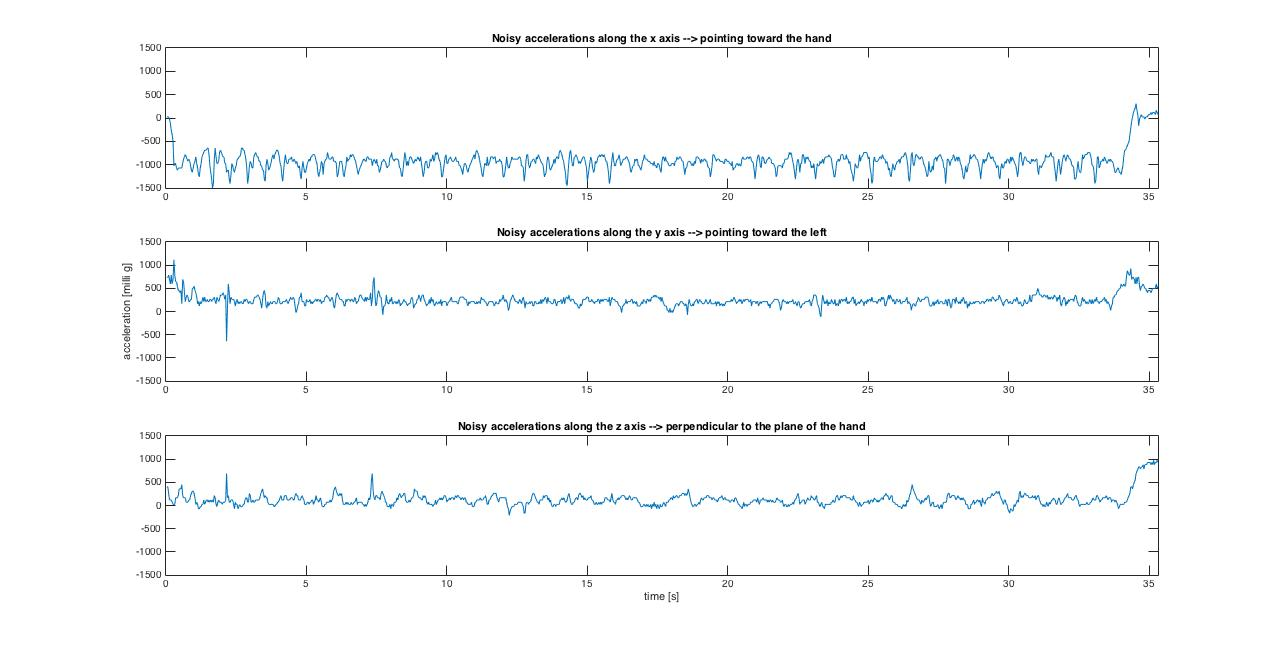
\includegraphics[width=0.8\linewidth]{../img/fig1.jpg}
   \caption{}
\end{center}
\end{figure}

By looking at the data, we can find that the period is around $0.7s$. Moreover, we noticed that the signal is pretty noisy, and a low pass filter might be useful for future processing. To find out a proper cutoff frequency, we did Fourier transform on the raw data, along its $x$ axis, resulting the following image:

\begin{figure}[t]
\begin{center}
%\fbox{\rule{0pt}{2in} \rule{0.9\linewidth}{0pt}}
   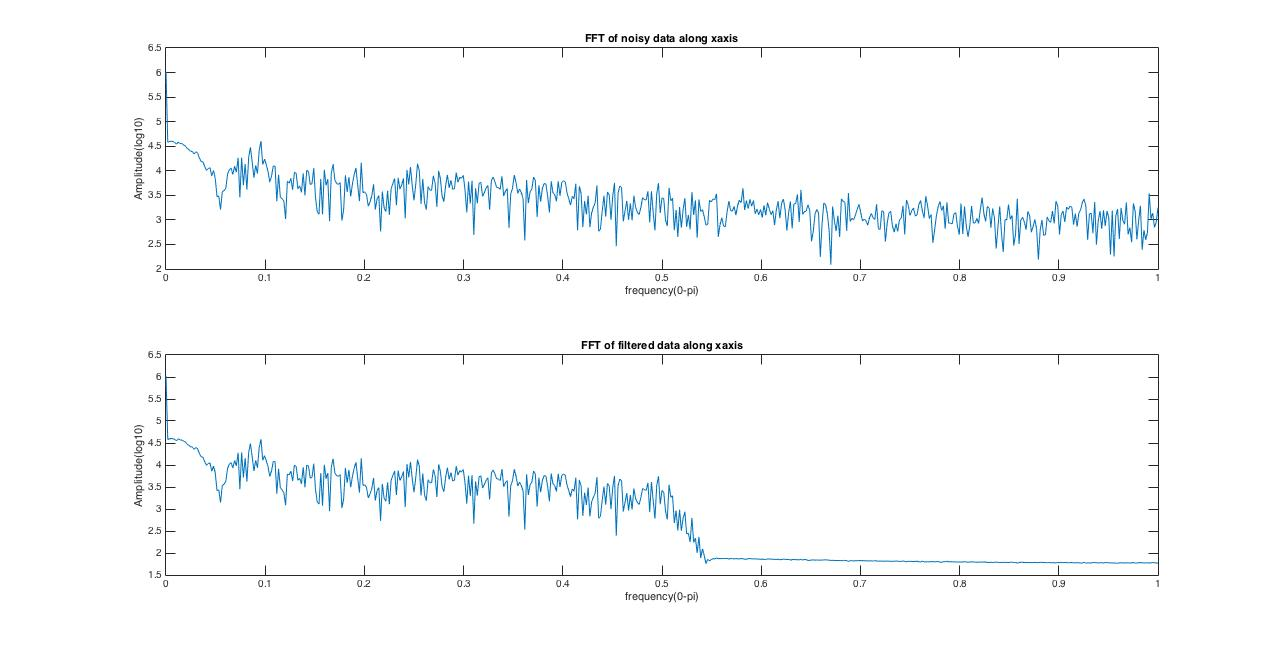
\includegraphics[width=0.8\linewidth]{../img/fig2.jpg}
   \caption{}
\end{center}
\end{figure}

By observing this image, the fundamental frequency is around $0.1\pi$, while the envelop is descending with ascending frequency. Taking a reasonable frequency diversity of different individuals into account, we finally set the cutoff frequency to $0.3\pi$. While a group delay is produced by passing data through a finite duration low pass filter, a trivial step is needed to remove this group delay. The filtered data shown below:

\begin{figure}[t]
\begin{center}
%\fbox{\rule{0pt}{2in} \rule{0.9\linewidth}{0pt}}
   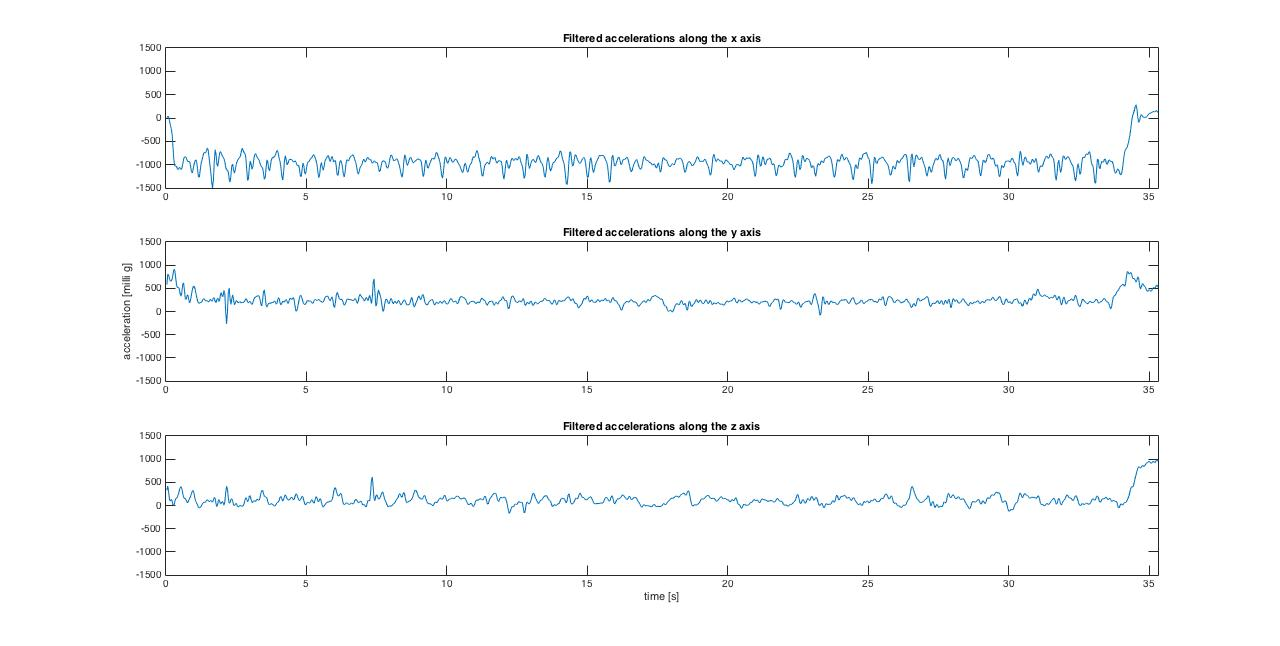
\includegraphics[width=0.8\linewidth]{../img/fig3.jpg}
   \caption{}
\end{center}
\end{figure}

Along with noise reduction, slow changing offsets in the signal must be removed.  Observing figure 5 it is clear that the signal is slowly drifting which could

\begin{figure}[t]
\begin{center}
%\fbox{\rule{0pt}{2in} \rule{0.9\linewidth}{0pt}}
   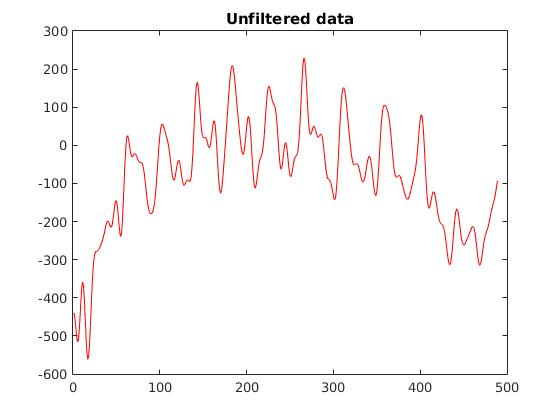
\includegraphics[width=0.8\linewidth]{../img/fig4.jpg}
   \caption{}
\end{center}
\end{figure}

lead to issues in later stages.  Bringing the data through a simple high pass filter with a cutoff of $0.25 Hz$ allows us to remove the offending drift without compromising the information in the data which is closer occurring at $1Hz$ or faster leaving us with the signal seen in figure 6

\begin{figure}[t]
\begin{center}
%\fbox{\rule{0pt}{2in} \rule{0.9\linewidth}{0pt}}
   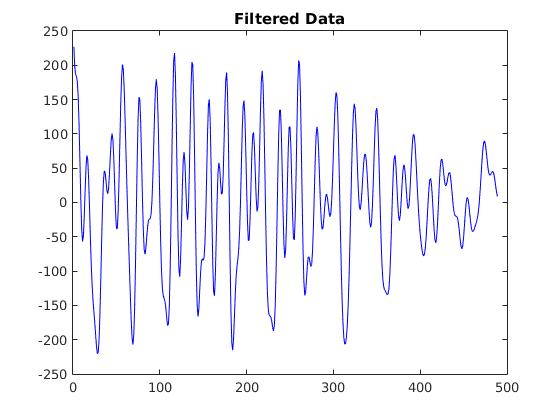
\includegraphics[width=0.8\linewidth]{../img/fig5.jpg}
   \caption{}
\end{center}
\end{figure}

\subsection{PCA and Projection}

The data from the files is measured along 3 axis over time, however the data processing is targeted at 1 dimensional time signal.  In order to simplify further calculations the dimension of interest is extracted using PCA.  The 3 dimensional data is projected onto the primary eigenvector resulting in the 1 dimensional time signal we desire that has the majority of the movement information.  A 3 dimensional signal and its 1 dimensional projection are shown in the figures below:

\begin{figure}[t]
\begin{center}
%\fbox{\rule{0pt}{2in} \rule{0.9\linewidth}{0pt}}
   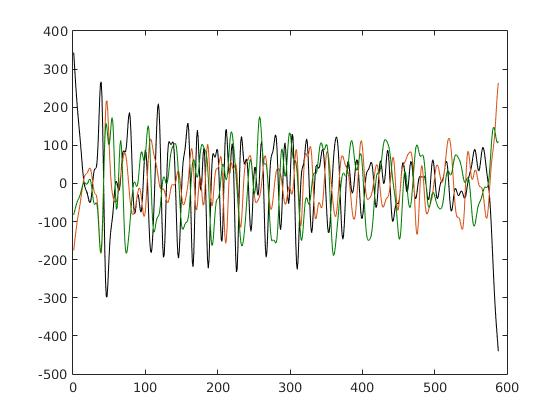
\includegraphics[width=0.8\linewidth]{../img/fig6.jpg}
   \caption{}
\end{center}
\end{figure}

\begin{figure}[t]
\begin{center}
%\fbox{\rule{0pt}{2in} \rule{0.9\linewidth}{0pt}}
   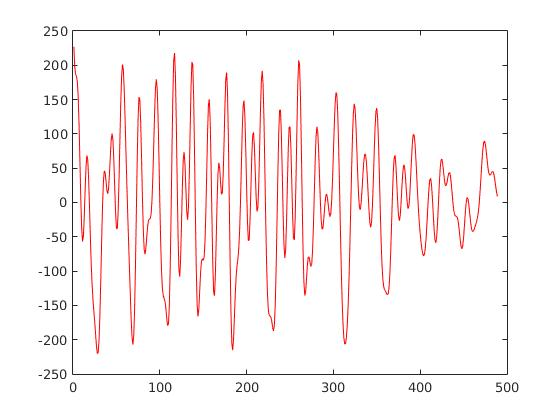
\includegraphics[width=0.8\linewidth]{../img/fig7.jpg}
   \caption{}
\end{center}
\end{figure}

As each person carries themselves differently the direction of this vector may also be telling as to who it is so this vector is saved to be a possible feature in further classifiers.

\subsection{Period Extraction}
Since walking can be approximated as a periodic movement of multiple body parts (legs cause bodies to move up and down; arms swing circularly with a certain period), we decided that the period of each dimension, and more importantly one full period of body movement along that dimension, are two important features that might help separate one person from another. To extract the period of a signal, we decided to employ the autocorrelation method, which computes the cross energy between a signal and its shifted copy. After that, we use the technique called non-local maximum suppression to sharpen the peak of the correlation output. As an alternative method, we used an FIR Gaussian filter to compute correlation, and the result shows better precision with faster computation speed, thanks to the Fast Fourier Transform.

%-------------------------------------------------------------------------
\subsection{MACE Filtering for Individual Verification}
To deal with pattern verification regardless of variations between different trials of the same individual, correlation seems to be a natural choice. As the first thought, a matched filter seems to be a choice. Matched filter is basically a template pattern that with training patterns as input, the correlation result will be at the pre-specified level, meaning ‘matched’. It is good for detecting the known reference with additive white Gaussian noise, but it’s not robust with even slight distortion of the data. 

Another correlation method to be considered is MACE(Minimum Average Correlation Energy) filter~\cite{Author01}. As it minimizes the average energy of the correlation outputs while maintaining high correlation with origins, it will has better discrimination performance. 

Testing vectors are normalized, to avoid correlation result confusion since different individuals might have considerable amplitude differences on accelerometer data.

\subsection{Other Classification Methods}

We consider trying the following methods for the optimal classification scheme:
\begin{itemize}
\item LDA
\item KNN clustering
\item Adaboost Classifier
\item Gaussian Mixture Model

\end{itemize}
After extracting features discussed above, (mace filter output, period, etc.) we will have a feature vector with a lot of information that identifies a person.  To find which of these features does the best at separating individuals, the listed classifiers will be used tried and the results of each compared.  LDA is trained on labeled data finding the lower dimensional space where they are maximally separated.  Adaboost looks at each dimension of the feature vector iteratively and chooses the single best one giving it a weight. This process is repeated over and over until a nonlinear decision boundary is chosen. KNN saves an instance of every data-point and new points are compared against them to find which of the classes has the majority of the closest points.  Gaussian Mixture models assume the data can be modeled as a sum of Gaussian probability distributions and finds the best parameters to do so.  Once modeled the new data-points are compared to the distribution to determine which class it best belongs in.  We suspect that since the feature vector is a series of many unrelated features that GMM and KNN will not work great and a solution like Adaboost will give us the best results.

%------------------------------------------------------------------------
\section{Database}

Dataset was found from UCI Machine Learning Repository~\cite{Author02}, called ‘Dataset for ADL Recognition with Wrist-worn Accelerometer Data Set’. In this dataset, there are recordings of 16 volunteers performing 14 Activities of Daily Living(ADL) while carrying a wrist-worn tri-axial accelerometer. These 14 activities include brush-teeth, climb-stairs, comb-hair, descend-stairs, drink-glass, eat-meat, eat-soup, getup-bed, liedown-bed, pour-water, sitdown-chair, standup-chair, use-telephone, and walk.

For now, we are using $walk$ as the only label for individual verification. In the future, we need to add more labels to perform simple activity identification before running individual verification. Moreover, we plan to use data collected by our own using Pebble watch and Android device, to apply the method used in this project in real world.

The $walk$ activity is identified as taking a number of steps, and there are 100 entries labeled $walk$ which are contributed by 10 volunteers; each entry contains 3 columns -- the first one represents x axis, which is pointing toward the hand; the second one is y axis pointing toward the left; the last one is $z$ axis and it’s perpendicular to the plane of the hand.

The range of data is from $-1.5g$ to $1.5g$, which is encoded using a linear mapping with an encoded data range of 0 to 63 inclusive. The sensitivity is 6 bits per axis and the sampling rate is $32Hz$. Following is a snippet in the dataset:\newline
...\newline
24 44 33\newline
21 46 32\newline
10 55 32\newline
11 48 32\newline
...\newline

%------------------------------------------------------------------------
\section{Results}
\subsection{Current}
    \begin{itemize}
    \item \textbf{Period Extraction}\newline
    Periods are extracted as described in the Method section, and here are some sample results with all period are resampled at a length of 50 samples, to have the same dimension as we’ll feed following steps like MACE filter with equal dimension input.

\begin{figure}[t]
\begin{center}
%\fbox{\rule{0pt}{2in} \rule{0.9\linewidth}{0pt}}
   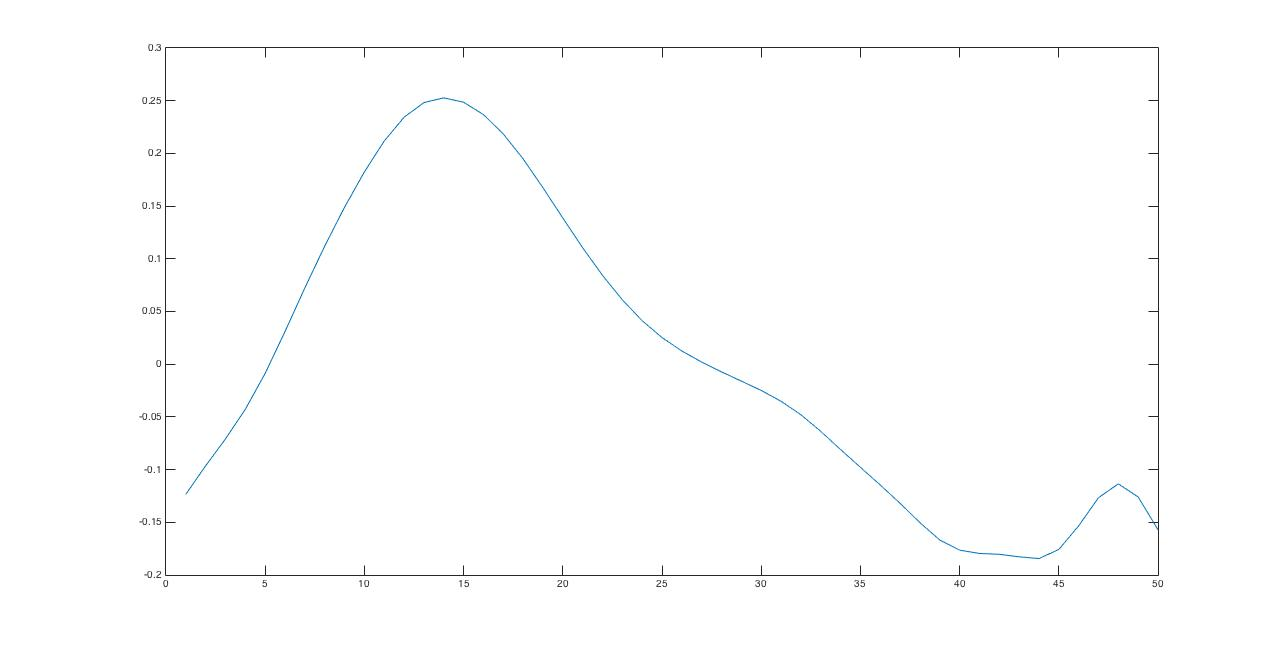
\includegraphics[width=0.8\linewidth]{../img/fig8.jpg}
   \caption{}
\end{center}
\end{figure}

\begin{figure}[t]
\begin{center}
%\fbox{\rule{0pt}{2in} \rule{0.9\linewidth}{0pt}}
   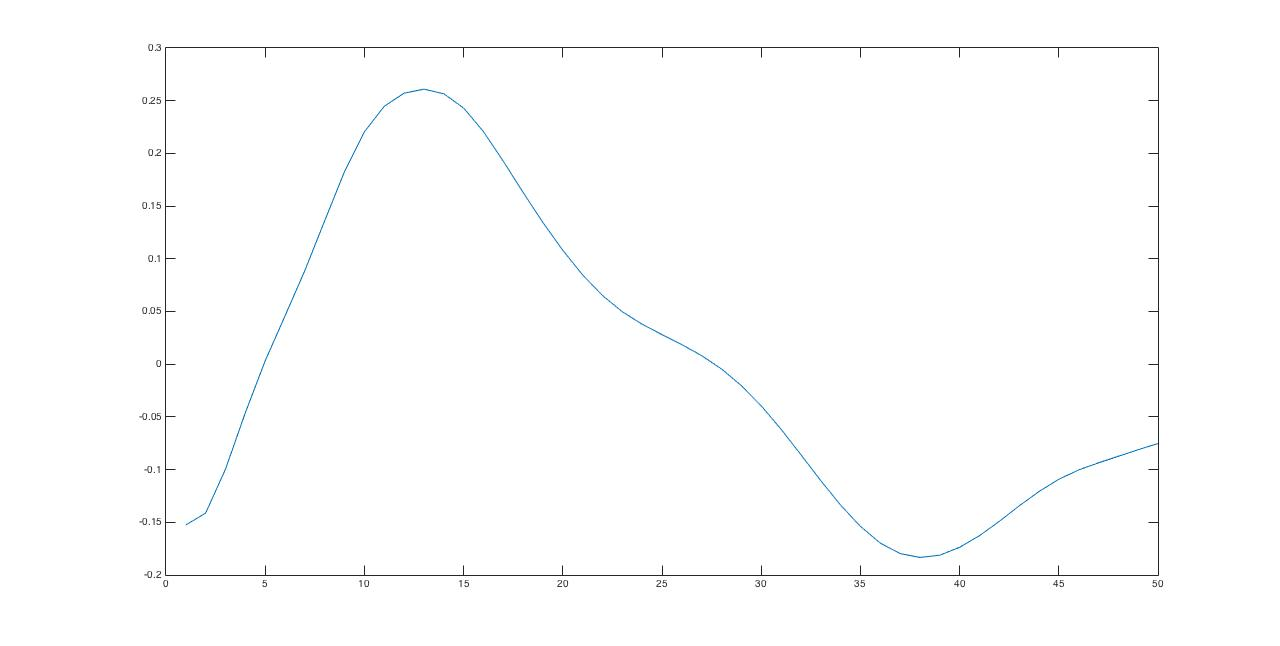
\includegraphics[width=0.8\linewidth]{../img/fig9.jpg}
   \caption{}
\end{center}
\end{figure}
\item \textbf{MACE Filter}\newline
The current result of MACE filter is pretty weak, which might implies that MACE filter is not as robust and generative as expected. MACE filter correlation result is as follows:

\begin{figure}[t]
\begin{center}
%\fbox{\rule{0pt}{2in} \rule{0.9\linewidth}{0pt}}
   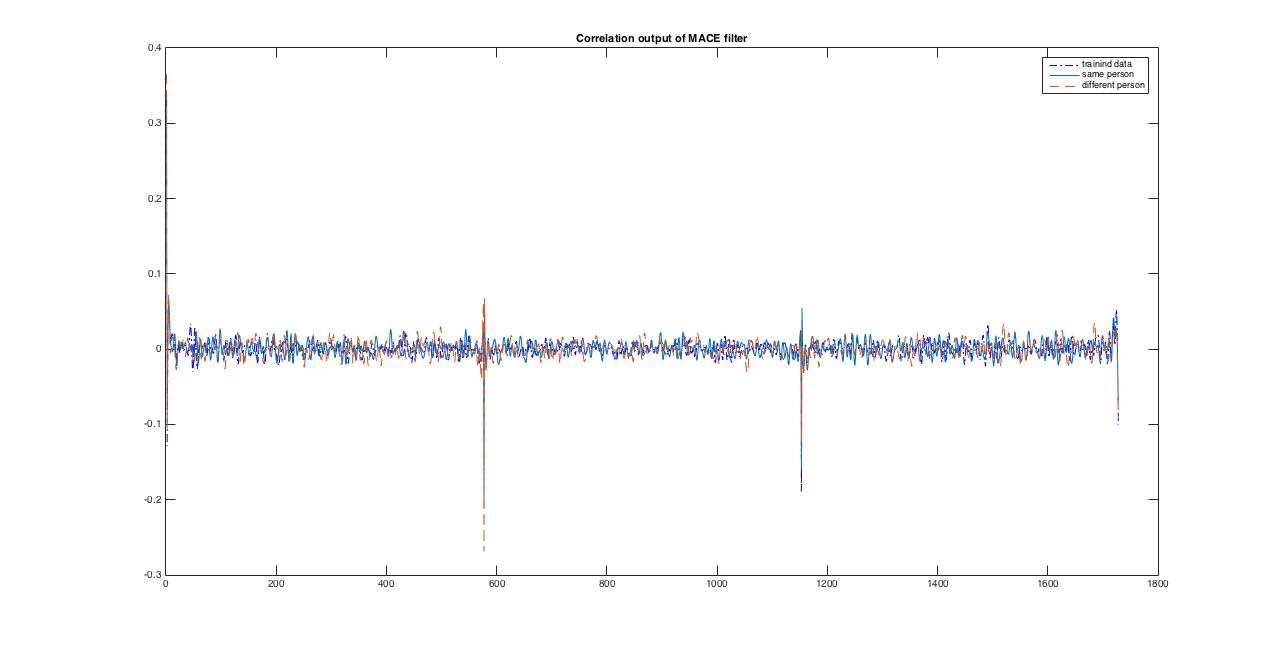
\includegraphics[width=0.8\linewidth]{../img/fig10.jpg}
   \caption{}
\end{center}
\end{figure}

For now, the input training vectors of MACE filter are whole trials, which involving multiple periods. The correlation result is considered to be improved by training the MACE filter on a period basis.
    \end{itemize}

\subsection{Expected}

%------------------------------------------------------------------------
\section{Comparison with Other Work}
Gait authentication by the means of pattern recognition is a novel idea. However, several workers have made the attempt to solve this problem with promising result. In their paper ~\cite{Author03}, Gafurov et al used three accelerometers to capture the accelerations along the X, Y, and Z dimensions. Then, they combined this three-dimensional data to calculate a more reliable combined acceleration signal. They further defined two features as functions of the combined acceleration signal, namely histogram similarity and cycle length, and used them as the features for their classifiers. So far, we have not reached the classification stage, so we have nothing to compare with their classification accuracy. Nevertheless, our ultimate goal is to reach comparable classification accuracy to the work mentioned above.

{\small
\bibliographystyle{ieee}
\bibliography{egbib}
}
\end{document}
